%\tiny
%\scriptsize
%\footnotesize
%\small

%\documentclass[submit,techrep]{ipsj}
%\documentclass[submit,techrep,noauthor]{ipsj}
\documentclass[submit,techrep,noauthor]{ipsj}

%\usepackage[dvips]{graphicx}
\usepackage[dvipdfmx]{graphicx,hyperref}
\usepackage{latexsym}
\usepackage{color}
\definecolor{blue}{rgb}{0.00, 0.00, 1.00}
\usepackage{listings}
\usepackage{amsmath}
\lstset{
language={C},
%basicstyle={\ttfamily},
basicstyle={\footnotesize},
numbers=left,
stepnumber=1,
breaklines=true,
lineskip=-0.5mm,
%xleftmargin=2zw,
frame={tb}, 
showtabs=false,
%formfeed={\hfill},
}
\usepackage{cite}
%	\usepackage{comment}
%	\usepackage{caption}
\def\newblock{\hskip .11em plus .33em minus .07em}

\def\Underline{\setbox0\hbox\bgroup\let\\\endUnderline}
\def\endUnderline{\vphantom{y}\egroup\smash{\underline{\box0}}\\}
\def\|{\verb|}

\setcounter{巻数}{53}%vol53=2012
\setcounter{号数}{10}
\setcounter{page}{1}


\begin{document}

\title{PMlibを用いた計算性能測定と性能可視化手法}

\affiliate{AICS}{理化学研究所 計算科学研究機構}
\paffiliate{Kyushu}{九州大学 情報基盤研究開発センター}

\author{三上 和徳}{Kazunori Mikami}{AICS}[kazunori.mikami@riken.jp]
\author{小野 謙二}{Kenji Ono}{AICS,Kyushu}[keno@cc.kyushu-u.ac.jp]

\begin{abstract}
オープンソースライブラリPMlib
を用いたアプリケーションの性能評価手法について報告する.
HPCシステムの仕様上の最大計算性能と
アプリケーション実行時に達成される実行性能との間には,様々な要因により
乖離が生じる.
この違いを議論する場合には,演算器の並列性やメモリ・キャッシュ各階層間
のデータ移動性能などのハードウエアの動作特性を中心に評価する視点と,
%局所性の確保はソフトウエアの話なのですか?
アプリケーションがソースプログラムレベルで要求する数値計算上の計算量と
コンピュータシステムが実際に実行する命令に基づいた計算量との違いを
評価する視点がともに有効である.
PMlibは数値計算上の計算量を明示的に測定する機能と,HWPCが記録する計算量を
測定する機能とを有し,両者の違いを定量的に評価することを可能とする.
またHWPC測定時には内部でPAPI低レベルAPIを利用し,
一般に選択と解釈が容易ではない各種ハードウエアイベント統計情報を
カテゴリ分けしてアプリ利用者が評価しやすい情報として選択出力する.
%
%	出力情報としてはアプリ実行中に蓄積された性能統計情報を時間平均化した
%	標準レポートの他,
%	性能統計情報を時系列出力してWebブラウザパッケージとの連携利用により
%	可視化する機能を持つ.
%
これらの異なる基準での計算量あるいは計算命令の実行状態を統計的に
評価することによって,
アプリケーションのHPCシステムにおける実行性能発現を理解する
一助とすることが可能である.

本報告ではPMlibを用いたアプリの性能評価手法を説明し,Intel Xeonサーバ
および富士通FX100上での評価事例を紹介する.
\end{abstract}

\maketitle

%	最後に句読点の変換を行う.全角.ー>全角.に,また全角,ー>全角,に
%	:1,$s/。/./g
%	:1,$s/、/,/g

\section{はじめに}
研究の目的

計算科学アプリケーションの開発および利用の各局面において,
利用するHPCシステム上で性能評価作業を実施することが頻繁に行われる.
これは主に,アプリケーションの性能特性を把握した後,ソフトウエア上の
最適化を実施して高速処理を実現するための可能性を探るために行われる.
このような性能評価作業が頻繁に実施される背景として,
HPCシステムの仕様上の最大性能とアプリケーションが実際に達成する実行性能との
差が,アプリの種類によっては非常に大きいことがある.

最大性能と実行性能との違いに関して
演算器の並列性やメモリおよびキャッシュ階層構成における局所性などの
ハードウエアの動作特性と関連づけられて
多くの研究が行われている.

アプリケーションがソースプログラムレベルで要求する数値計算上の計算量と,
コンピュータシステムが実際に実行する命令を HWPC(ハードウエア性能カウンタ)
で測定した計算量との間ではしばしば乖離がある.
この事は性能評価において重要な問題点として考慮されなければならない.

PMlibは数値計算上の計算量を明示的に測定する機能と,HWPCが記録する計算量を
測定する機能とを有し,両者の違いを定量的に評価することを可能とする.
HWPC測定には内部でPAPI低レベルAPIを利用し,
一般に選択と解釈が容易ではない各種ハードウエアイベント統計情報を
カテゴリ分けしてアプリ利用者が評価しやすい情報として選択出力する.

出力情報としてはアプリ実行中に蓄積された統計情報を時間平均化した
標準レポートに加え,
経過時間軸に沿った動的な情報の出力も可能であり,
計算性能の時系列挙動を可視化するWebブラウザパッケージとの連携利用
が可能な構成となっている.

本報告ではまず計算科学的観点での計算量とシステム評価的観点での計算量との違い
についていくつかの評価事例を示す.

次に,計算量から計算性能を求める段階で,その性能を律速する
ハードウエアの動作特性を読み取るPMlibの機能について事例を示す.



\section {計算量と性能評価}
\label{section:computing-volume}

\subsection {計算科学的観点での性能}
\label{subsection:scientific-perf}
計算量という用語を用いる場合,計算科学アプリケーションの開発者は,
Fortran言語やC++言語などで記述されたソースプログラム上で計上される
数値計算量すなわち演算回数の合計値としての
計算量\begin{math} OP \end{math}は以下の式で表わされる.
%	\begin{math}
%	\end{math}
%単純結合式
\begin{align*}
OP_{source} = \#add + \#sub + \#mult + \#div \\
	+ \#max + \#sqrt + ...
\end{align*}

ソースプログラムで記述される四則演算や基本的な数学関数ごとそれぞれに
計算の「重たさ」が異なるため,アプリケーションの計算負荷としては
その「重たさ」を係数
\begin{math} c_{op} \end{math}
として考慮した以下の式で計算量を表現することができる.
% OP_{system}
\begin{align*}
OP_{weight} =
	c_{add}\times \#add + c_{sub}\times \#sub + c_{mult}\times \#mult \\
	+ c_{div}\times \#div + c_{max}\times \#max + c_{sqrt}\times \#sqrt + ...
\end{align*}

計算性能はこの計算量を計算経過時間で割った値として定義される.
\begin{align*}
Perf = OP / Time	% \div はあまり見た目が良くない,,,
\end{align*}

HPCアプリケーションにおいて
所与の計算を効果的に達成するために計算時間の短縮をめざす場合,
必要な計算量を削減するアルゴリズムを開発・採用するというアプローチ
が多いが,そのような場合の計算量とは主に上記した
計算科学的観点での評価が意図される.
このような計算科学的観点での計算性能を以降数値計算性能と呼ぶことにする.

HPCシステムの性能評価に長く利用されてきたLinpack(HPCC)が出力する
Gflops値も加算・乗算の「重たさ」を等しく1として上記結合式を評価した
計算量から,計算性能を次式で求めている.
\begin{align*}
Gflops = N^{2} \times ( 2/3 * N + 3/2 ) \times 1.0^{-9} / Time 
\end{align*}



\subsection {システム評価的観点での性能}
\label{subsection:system-perf}

アプリケーションをHPCシステム上で実行する段階では,
ソースプログラムを言語コンパイラを通して生成した実行プログラムの
機械語命令列としてスケジューリング処理することになる.
ソースプログラムでは単純な計算式であっても,実際に実行されるのは
複数の命令列であり,命令の種類・量・命令に対応する計算量(演算数)は,
実行するHPCシステムのアーキテクチャおよびコンパイラなど
言語処理系ソフトウエアの最適化水準に依存する部分が大きい.

HPCシステムが実際に処理するこの計算量を経過時間で割った値が
システム評価的観点での計算性能として定義される.

この計算量を測定するためには,HPCシステムに通常装備されている
HWPC(Hardware Performance Counter)に記録されるイベントカウント数
を利用することが可能である.
適切なAPIによってHWPCに記録された情報へアクセスし,
実行された命令数を測定して計算量を求める.

例えば後出のIntel Xeon Skylake Goldプロッセサの浮動小数点演算に属する計算量は
HPWCで計上されたイベント数を基にして以下の式により求められる.

\begin{math}
fpsp1  : "FP\_ARITH:SCALAR\_SINGLE"; \\
fpsp4  : "FP\_ARITH:128B\_PACKED\_SINGLE"; \\
fpsp8  : "FP\_ARITH:256B\_PACKED\_SINGLE"; \\
fpsp16 : "FP\_ARITH:512B\_PACKED\_SINGLE"; \\
fpdp1  : "FP\_ARITH:SCALAR\_DOUBLE"; \\
fpdp2  : "FP\_ARITH:128B\_PACKED\_DOUBLE"; \\
fpdp4  : "FP\_ARITH:256B\_PACKED\_DOUBLE"; \\
fpdp8  : "FP\_ARITH:512B\_PACKED\_DOUBLE";
\end{math}
\begin{align*}
OP{hwpc} = fpsp1 + fpdp1 + 4.0*fpsp4 + 8.0*fpsp8 \\
	+ 16.0*fpsp16 + 2.0*fpdp2 + 4.0*fpdp4 + 8.0*fpdp8;
\end{align*}

富士通FX100のプロッセサであれば, \par
\begin{math}
fpdp1  : "1FLOPS\_INSTRUCTIONS"; \\
fpdp2  : "2FLOPS\_INSTRUCTIONS"; \\
fpdp4  : "4FLOPS\_INSTRUCTIONS"; \\
fpdp8  : "8FLOPS\_INSTRUCTIONS"; \\
fpdp16 : "16FLOPS\_INSTRUCTIONS";
\end{math}
\begin{align*}
OP{hwpc} = fpdp1 + 2.0*fpdp2 + 4.0*fpdp4 \\
	+ 8.0*fpdp8 + 16.0*fpdp16; 
\end{align*}

このように測定される計算量を以下,HWPC計算量とよび,HWPC計算量を基準とした
計算性能をHWPC計算性能と呼ぶことにする.
いわゆるシステム性能に主眼がおかれた文脈で使用されることが多い.

HWPC測定性能が高く表示されるにもかかわらず,
数値計算上の性能は低いという状況は,
本節で述べた観点が違う事による計算量の定義の違い,
および
ハードウエアの有効利用の状況
の双方の影響を受けた結果であるといえる.


\section{PMlib}

\subsection {PMlibについて}

PMlibはアプリケーションの計算性能モニター用のクラスライブラリであり,
オープンソースソフトウエアとして公開されている.
\cite{PMlib2:webpage} \par
PMlibは前述した2種類の計算性能(数値計算性能とHWPC計算性能)
を測定する機能を持つ.
アプリのソース中に測定区間を指定して,
測定区間毎の統計情報をアプリ終了時・あるいは計算途中の指定位置で出力する.

測定区間は区間の名称,測定計算量の種類(演算量|データ移動量),
排他性(排他的|非排他的),蓄積計算量からなる少数の属性を持つ.
アプリ終了時の出力レポートに測定区間単位,プロセス単位,アプリ単位での
計算性能が表示される.
出力する情報の内容はアプリ実行時のオプションとして環境変数を指定する事によ
り制御される.


\subsection {PMlib APIの利用}
PMlibはC++およびFortranプログラムから呼び出して利用することができる.
以下
%\ref{listing1}
はPMlib APIを利用するFortranソースプログラムの例である.
% \begin{lstlisting}[caption={FortranプログラムへのPMlib組み込み例}]
% \begin{lstlisting}[caption={\hfill},label={listing1},captionpos=t]
\begin{lstlisting}
program main
call f_pm_initialize (nWatch)
call f_pm_setproperties ("Section1" icalc, iexcl)
call f_pm_start ("Section1")
call MyComputation (fops)	!cx measured computation
call f_pm_stop ("Section1", fops, ncall)
call f_pm_print ("", isort)
call f_pm_printdetail ("", ilegend, isort)
end
\end{lstlisting}


\subsection {測定する計算量の指定}
数値計算上の計算性能を測定したい場合は,
PMlib APIの引数として該当区間の計算量を評価式の形で明示的に指定して積算する.
ソースプログラムに記述された計算式の全計算回数を数え上げる事に等しい.
その際に計算の種類ごとの「重たさ」の設定は任意である.

HWPC測定値を基準とした(システム評価的観点での)計算性能を測定したい場合は,
該当区間のHWPCイベント統計情報をPMlibに読み取らせ
計算量を積算させるため,APIへ引数として渡される値は用いられない.
HWPCの読み取りには内部でPAPI低レベルAPIを利用し,
アプリ利用者が評価しやすい情報として自動的に選択出力する.

HWPCイベントをアプリから直接 PAPI APIでアクセス利用するのは一般に
容易ではない.プリセットされた基本的なHWPCイベントだけではなく,
より詳細なHWPCイベントを選択抽出するために,nativeイベント群と
そのマスクを調査する必要がある.
例えば後出のSkylake Goldプロッセサを搭載したサーバで
papi\_native\_avail コマンドの出力を確認すると5000行以上の情報が出力され,
その出力からプロセッサアーキテクチャに依存する
注目する計算性能(計算量)を構成するにイベント名とイベントコードを調査し,
少数の物理的なカウンターに選択登録するするだけでも相当な負担である.

PMlibを組み込んだアプリケーションでは環境変数 HWPC\_CHOOSER を
右のカテゴリ値のどれかに設定すると,上記のような調査・妥当なHWPCイベント
の選択登録などを内部で実施し,計算量の統計を収集することができる.
カテゴリ値:
FLOPS \textbar BANDWIDTH\textbar VECTOR\textbar CACHE

%	PMlibの出力レポート例

PMlibではプロセス単位で性能情報を取得する設計となっていて,
プロセスがOpenMPスレッドを発生する場合,各スレッドの性能情報は帰属する
プロセスに集計される.

PMlibは一時的なベンチマークツールというよりは,アプリに常時組み込んで
プロダクション利用することを想定したライブラリである.

\subsection{PMlibの内部タイマー}
PMlibは移殖が容易な汎用のパッケージであり,デフォルトではLinuxの標準タイマー
であるgettimeofday関数を利用するが,HPCシステムがオーバーヘッドの少ない
高解像度タイマーを有している場合や,タイムスタンプカウンタを直接
アクセスできる場合は,それを利用するバージョンをビルドできるパッケージング
を目指している.
前節で示したHPCシステムでそのようなオプションを利用できる.
図\ref{fig:precise-timer} は標準タイマーを使用した場合と
高性能タイマーを使用した場合とのタイマー自身の測定解像度の比較である.

\begin{figure}[bt]
\centering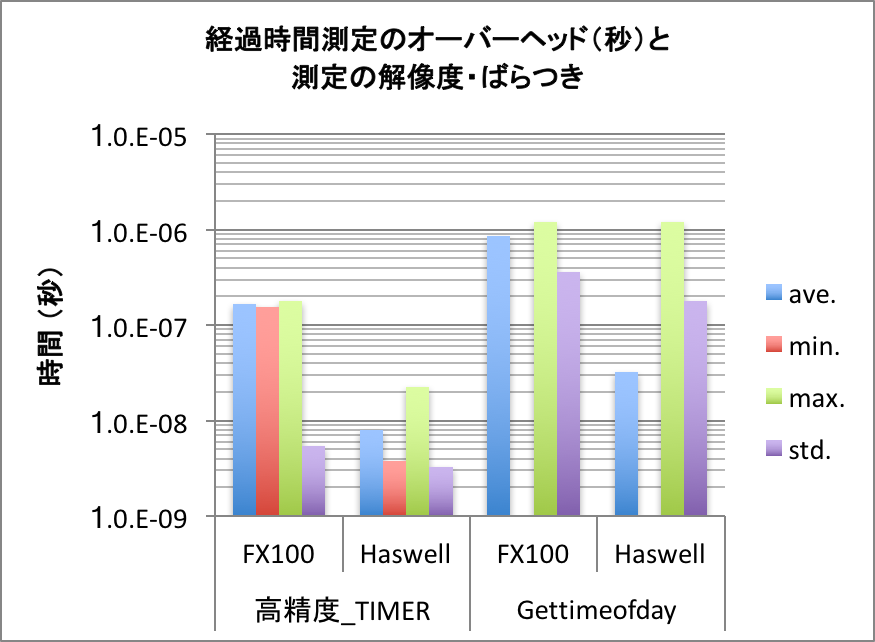
\includegraphics[width=0.45\textwidth]{figs/precise-timer.png}
\caption{precise-timer}
\label{fig:precise-timer}
\end{figure}



\subsection{PMlibの出力情報}
PMlibの出力として,標準出力や指定ファイルへのテキストレポート,および
汎用のトレースフォーマットであるOTF(Open Trace Format)ファイルを出力
する機能を持っている.


\subsection{関連する性能評価ツールと関連研究}

HPCシステム向けに様々な性能評価のためのツールが公開あるいは販売されている.\par
オープンソース性能評価ツール類としては
\begin{itemize}
	\item Scalasca \cite{Scalasca:2017} : トレース生成,Score-P共通インフラ
	\item Extrae \cite{Extrae:webpage} : トレース生成
	\item PAPI \cite{PAPI:5.6} : HWPCへのアクセス
	\item Linux perf tools : HWPCへのアクセス
\end{itemize}
ベンダーが提供する性能評価ツール類としてはX86系では 
\begin{itemize}
		\item Intel VTune \cite{Intel:VTune}, PGI Profiler \cite{PGI:Profiler}
\end{itemize}
また各HPCシステムは通常専用の性能評価ツールを装備している.
\begin{itemize}
	\item FX100システムでは富士通プロファイラなど
\end{itemize}
それぞれに特徴があり,
ベンダー製品のツールはパッケージが統合化されて完成度が高い反面,
利用できるシステムが制限され,相当の習熟期間が必要となる.
オープンソースのツールは様々なシステムへの移植が可能であるが,
各ツール毎に特徴・機能が明確で複数のツールを組み合わせて使う場合が多い.

特筆すべき点は,これら既存のツールはほぼ全てが評価の基準を,
システム評価的観点での性能すなわちHWPC測定性能に拠っていることである.


\section{PMlibを用いた性能測定と分析例}


基本的な演算についてPMlibを用いた分析例を示す。


\subsection{性能測定プラットフォーム}

測定には以下のHPCシステムを用いた.
\begin{itemize}
{
%	\setlength{\itemsep}{-5pt}
%	\setlength{\topsep}{2mm}
\item Intel Ivybridge CPU搭載サーバ
\item Intel Skylake CPU搭載サーバ
\item 富士通prime HPC FX100
}
\end{itemize}

これらプラットフォームの主にCPU部分についての性能諸元を
表\ref{tab:server-config}に示す.
\newif\ifTwoservers
\newif\ifThreeservers
\Twoserversfalse
\Threeserverstrue
%\tiny
%\footnotesize
%\small
\begin{table}[b]
\scriptsize
\caption{サーバの構成と最大性能(主にCPU部分)}
\label{tab:server-config}
\footnotesize

\ifTwoservers
\begin{tabular}{l|c|c} \hline
\scriptsize
system			&	FX100	&	Skylake	\\ \hline
CPU				&	SPARC64 XIfx	&	Gold 6148	\\ \hline
core GHz		&	1.975	&	2.4	\\ \hline
core Gflops	&	31.6	&	〜30	\\ \hline
L1\$ size (D,I)		&	64KB, 64KB	&	32KB, 32KB	\\ \hline
L1D\$ BW GB/s	&	140/R+70/W	&	154/R + 77/W	\\ \hline
\$ Linesize 	&	256B	&	64B	\\ \hline
L2\$ size		&	-	&	1MB	\\ \hline
L2\$ BW GB/s/core	&	-	&	154 ( ~70)	\\ \hline
LL\$ size		&	12MB	&	28MB(1.4MB/c)	\\ \hline
LL\$ BW GB/s/core	&	70/R+35/W	&	77 ( ~43)	\\ \hline
Memory			&	HMC(8x16Ls)	&	DDR4-2666	\\ \hline
Mem GB/s/[CMGcpu]	&	120/R+120/W	&	128	\\ \hline
\#cores/[CMGcpu]	&	16	&	20	\\ \hline
\end{tabular}
\fi

\ifThreeservers
\begin{tabular}{l|c|c|c} \hline
\scriptsize
Symbol			&	FX100	&	SKY		&	IVY \\ \hline
Platform		&	FX100	&	Skylake & Ivybridge\\ \hline
CPU				&	SPARC64 XIfx	&	Gold 6148	&	E5-4620v2	\\ \hline
core GHz		&	1.975	&	2.4	&	2.6 \\ \hline
core Gflops	&	31.6	&	〜30	\\ \hline
\#core/cpu*	&	16	&	20	&	8	\\ \hline
L1\$ size(D,I)		&	64KB, 64KB	&	32KB, 32KB	\\ \hline
L1D\$ BW GB/s	&	140/R+70/W	&	154/R + 77/W	\\ \hline
\$ Linesize 	&	256B	&	64B	&	64B	\\ \hline
L2\$ size		&	-	&	1MB	&	256KB	\\ \hline
L2\$ BW GB/s/c	&	-	&	154 ( ~70)	\\ \hline
LL\$ size		&	12MB	&	28MB	&	20 MB	\\ \hline
LL\$ BW GB/s/c	&	70/R+35/W	&	77 ( ~43)	\\ \hline
Memory			&	HMC(8x16Ls)	&	DDR4-2666	& DDR3-1600	\\ \hline
Mem GB/s/cpu*	&	120/R+120/W	&	128	\\ \hline
\#cores/cpu*	&	16	&	20	\\ \hline
\multicolumn{4}{l}{\scriptsize\hspace{5mm} 注 cpu* はCPUまたはCMGを意図する}\\
\end{tabular}
\fi

\end{table}


\subsection{基本的な演算性能の評価}

基本的な演算として,四則演算と平方根の配列計算カーネルを評価する.
fortranソースプログラムの抜粋を以下に示す.

%	\begin{lstlisting}[label={listing3},captionpos=t]
%	\begin{lstlisting}[caption={\hfill},label={listing3},captionpos=t]
\begin{lstlisting}
subroutine sub_add(a,b,c,n)
real a(n), b(n), c(n)  
do i=1,n
c(i)=a(i)+b(i)
end do
return
subroutine sub_fma(a,b,c,n)
real a(n), b(n), c(n)  
do i=1,n
c(i)=a(i)+b(i)*d
end do
return
subroutine sub_divide(a,b,c,n)
real a(n), b(n), c(n)  
do i=1,n
c(i)=b(i)/a(i)
end do
return
subroutine sub_sqrt(a,b,c,n)
real a(n), b(n), c(n)  
do i=1,n
c(i)=sqrt(a(i))
end do
return
\end{lstlisting}
どの計算もストライド1の依存性のないループで行われるため,
効率の良いパイプライン化・SIMD化・ベクトル化処理が適用されると
期待されるものである.

上記ソースの各サブルーチンをメインプログラムから多数回呼び出して,
その平均値を得てから,サブルーチン呼び出し
オーバーヘッドの時間を差し引いて,計算に必要な時間を求める.
doループのオーバーヘッドは差し引かない.
占有状態で負荷変動が少ない小規模構成の環境で測定を行う場合は,
上記のような単純な方法で測定して問題ないが,
利用負荷が高い共用サーバなどの上で同様の結果を得るためには,
一般にOS,共有ファイルシステム,トポロジを共有するネットワーク,
などの様々な要因から時間変動があり,粒度の小さな計算において
そのようなノイズを除去することは容易ではない.
測定におけるノイズ成分を利用者側で除去する方法としては,
上記の多数回呼び出しループの外側にさらに10回程度反復する最外側ループを設け,
最外側10回測定値の内,標準偏差1σの範囲だけを採用する方法などが効果的である.

この演算カーネルの測定をループ長
\begin{math}
n=1,2,4,..,2^{26}
\end{math}
に対してFX100で実行した結果を図 \ref{fig:fx100-gflops-long-R8}に示す.
\begin{figure}[bt]
\centering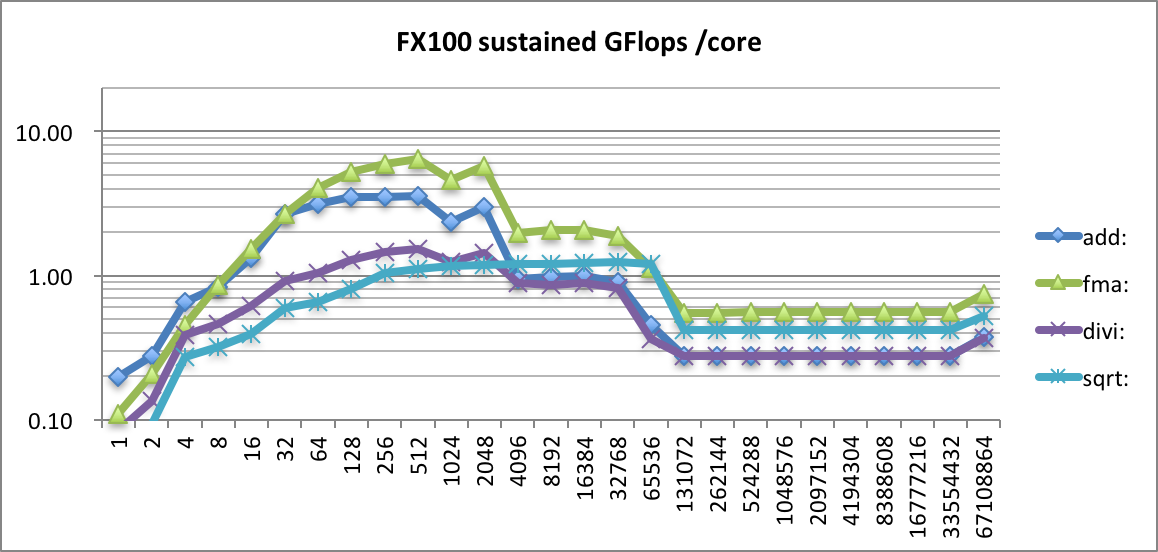
\includegraphics[width=0.45\textwidth]{figs/fx100-gflops-long-R8}
\caption{fx100-gflops-long-R8}
\label{fig:fx100-gflops-long-R8}
\end{figure}

表示しているのは数値計算上の性能である.
nの増加に連れてなだらかに性能が向上し,L1キャッシュ容量に収まる範囲で
最も高い性能に達し,その後L2キャッシュ容量の範囲内で,ついでメモリ
からのバンド幅で律速されるラインに落ち着くという全体傾向は,
従来の多数の関連研究結果と重なるものであり,
ループ長が長い部分においては roofline envelopの
L1\$ / L2\$ / LLC / メモリ各階層のバンド幅で段階的に律速されている.
ループ長が短い部分においてはループ処理自体のオーバーヘッドが
演算量に比して重く,アクセスレイテンシで律速されている.
\cite{Williams:2009:RIV:1498765.1498785} 

同じカーネルに対してループ長が短い部分で
nを連続的に変化させて測定した結果を
FX100 について図 \ref{fig:fx100-gflops-short-R8}に,
IVY について図 \ref{fig:ivy-gflops-short-R8}に各々示す.
nを1から128の範囲で連続的に変化させて測定した結果と
1から50の範囲をクローズアップした結果を示している.

\begin{figure}[bt]
\centering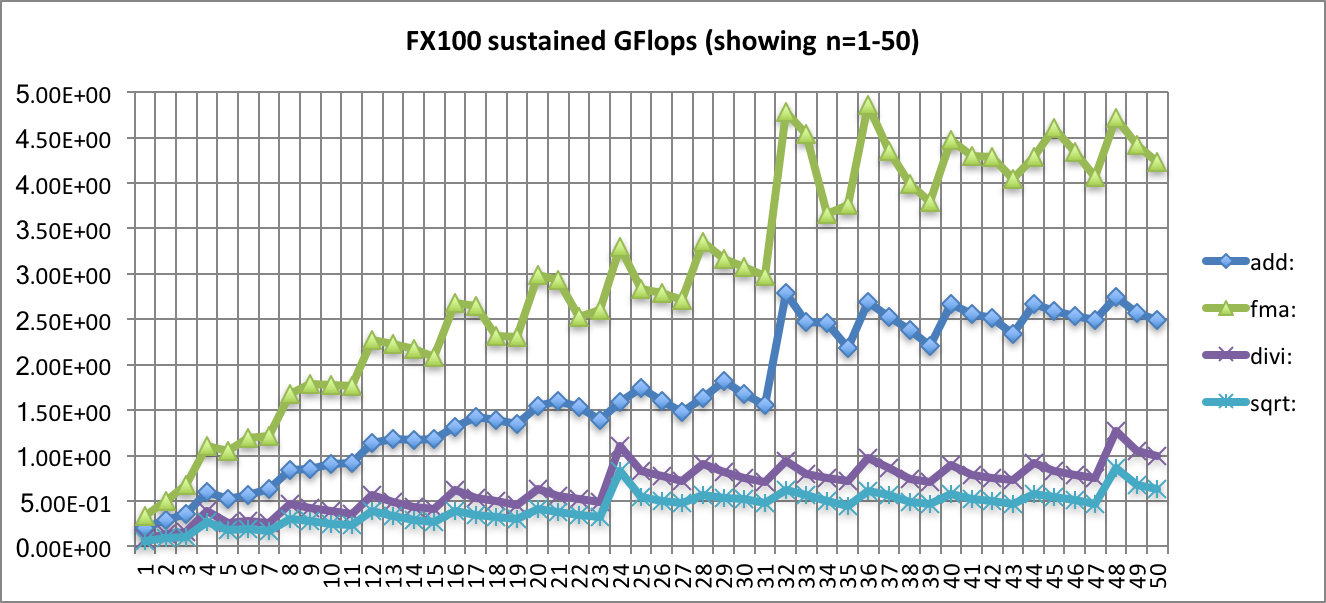
\includegraphics[width=0.45\textwidth]{figs/fx100-gflops-short-R8}
\caption{fx100-gflops-short-R8}
\label{fig:fx100-gflops-short-R8}
\end{figure}

\begin{figure}[bt]
\centering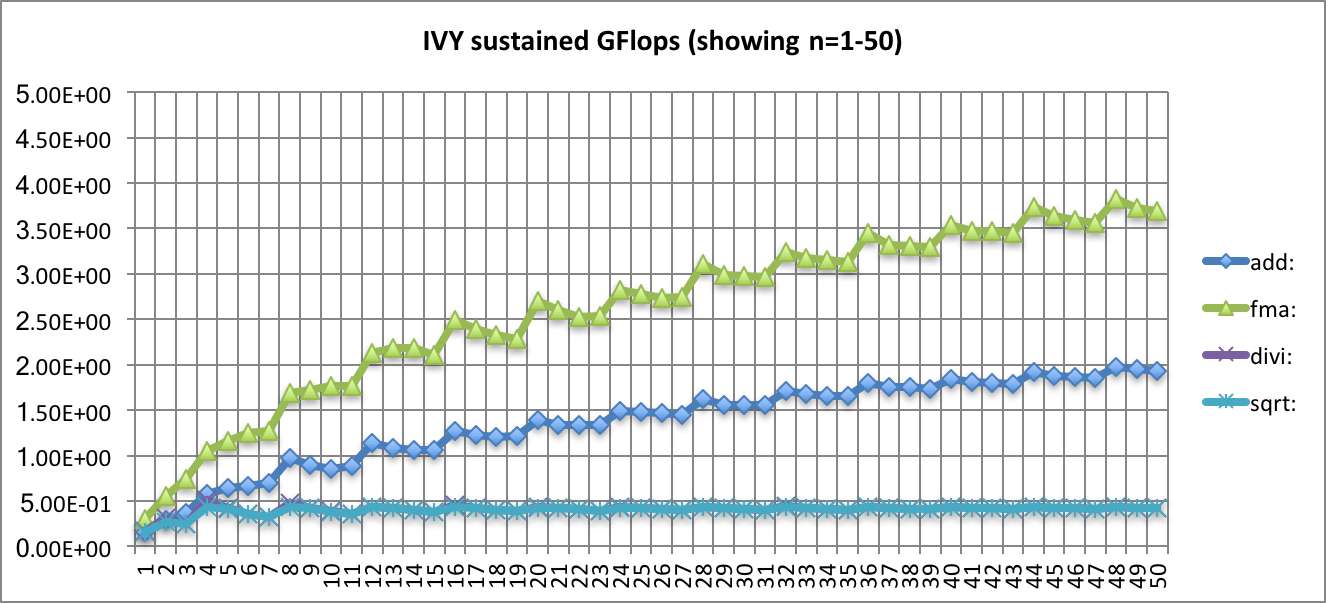
\includegraphics[width=0.45\textwidth]{figs/ivy-gflops-short-R8}
\caption{ivy-gflops-short-R8}
\label{fig:ivy-gflops-short-R8}
\end{figure}

Perfが単調に増加するのではなく,nが一定値の倍数において規則的に
向上する変動がみられるが,これは連続データに対して
SIMD化命令を適用した計算でよくみられる状況である.
この一定値はSIMD幅(SIMDビット数/データビット数)に対応するもので,
例えばFX100において倍精度(64ビット)計算を行う場合は
\begin{math}
256 / 64 = 4
\end{math}
であるため,計算性能は
4n,4n+1,4n+2,4n+3と低下した後,4(n+1)で再び向上する.

図 \ref{fig:fx100-gflops-short-R8}は
SIMD機構をもつシステム上でのプログラミングにおいては,
プログラムのループ長を該当アーキのSIMD幅の倍数となるような
コーディングを意識することが,
短いループ長の計算性能の向上においては特に重要であることを
示している.

単精度(32ビット)計算を行う場合はこの一定値は
\begin{math}
256 / 32 = 8
\end{math}
となり,さらに顕著な性能影響効果がみられる.
図 \ref{fig:fx100-gflops-short-R4}はFX100,
図 \ref{fig:HAS-gflops-short-R4}はHaswell CPUでの単精度計算
の性能状況を示している.

\begin{figure}[bt]
\centering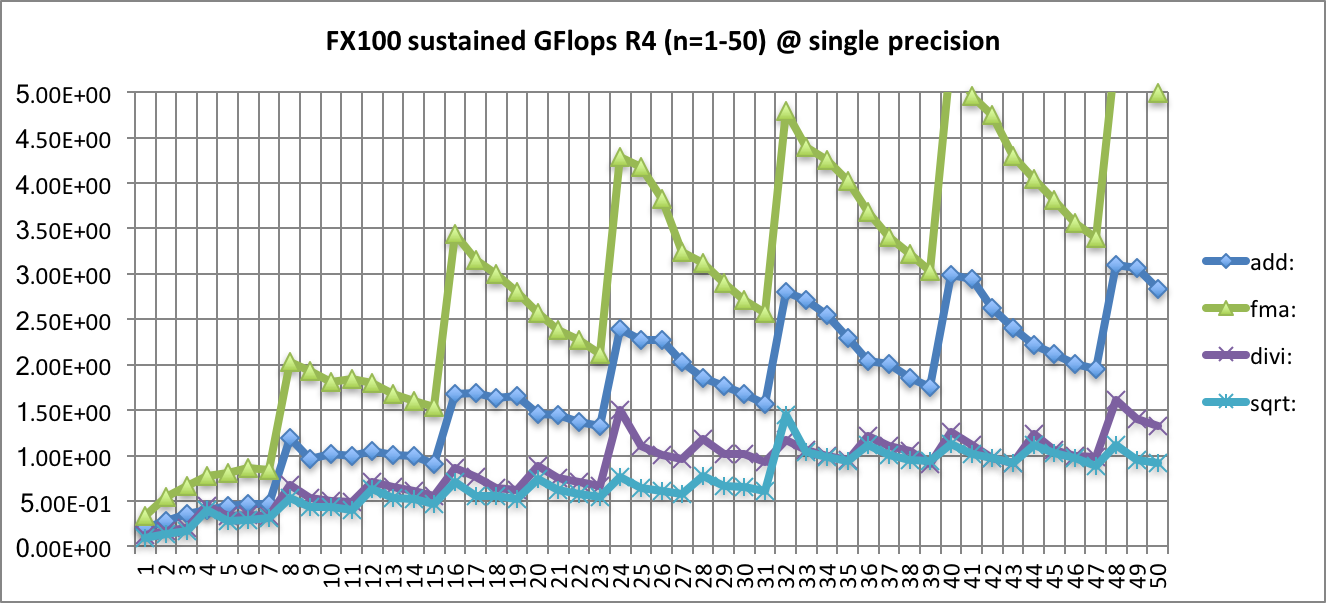
\includegraphics[width=0.45\textwidth]{figs/fx100-gflops-short-R4}
\caption{fx100-gflops-short-R4}
\label{fig:fx100-gflops-short-R4}
\end{figure}


\begin{figure}[bt]
\centering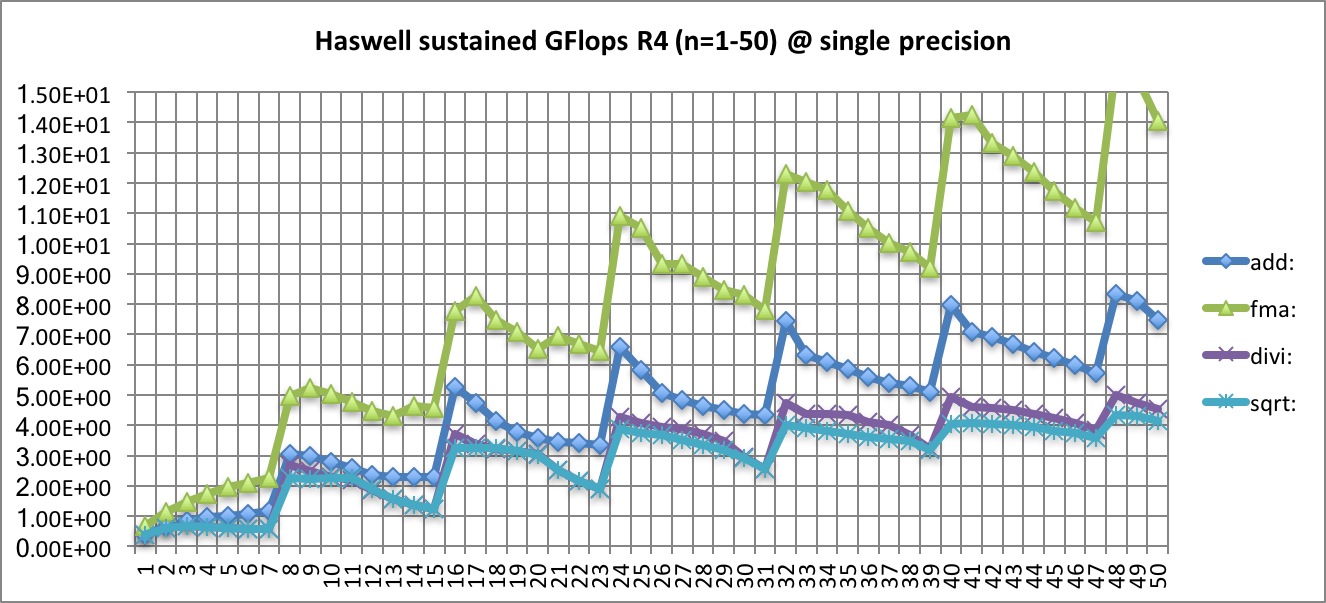
\includegraphics[width=0.45\textwidth]{figs/HAS-gflops-short-R4}
\caption{HAS-gflops-short-R4}
\label{fig:HAS-gflops-short-R4}
\end{figure}

PMlibを用いたプログラムの統計情報の出力および可視化によって、
このような性能特性の把握が可能となり、計算の高速化への指針の
一助が得られる。



\if0
\subsection{STREAM性能の評価}
STREAMベンチマーク\cite{stream:1995}
はコンピュータシステムのメモリバンド幅を測定するためのツールとして広く用いられている.
STREAMは変数配列の積和算(TRIAD)など,メモリread/write処理が主要な負荷となる
計算式の性能をアプリケーションプログラムレベルで測定出力する.
したがってその結果は「計算科学的観点」で評価された性能である.
このSTREAMプログラムを「システム評価的観点」で評価するとかなり様相が異なって来る.

まずSTREAMをSkylakeサーバ上で実行した場合の出力結果を示す.
Intelコンパイラのデフォルトオプションを用いている.
STREAM FortranプログラムOpenMPスレッド並列版を
1CPU上で8スレッド実行した場合,20スレッド実行した場合について示す.


Skylakeサーバ
されたHWPCベースでの
PMlibを用いて
メモリ階層での実測イベントベースによるデータ移動の状況を示す.
図



Intelコンパイラにはオプションが多数あり,中でも特にメモリバンド幅に関係が深いと
思われる以下のオプションを組み合わせて比較した結果を
図\ref{fig:stream-ivy-compact-1cpux8} に示す.\\
{\color{blue}この図は仮置きでIvybridgeの結果.Skylakeの結果と差し替えること.}

\begin{figure}[bt]
\centering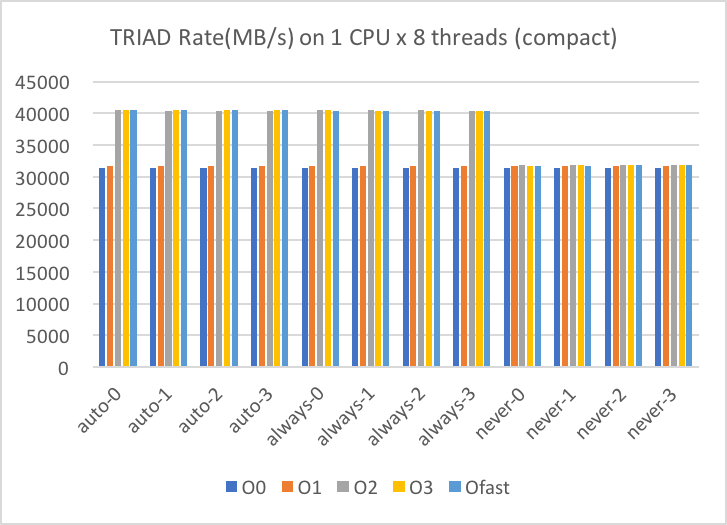
\includegraphics[width=0.45\textwidth]{figs/stream-ivy-compact-1cpux8.png}
\caption{stream-ivy-compact-1cpux8}
\label{fig:stream-ivy-compact-1cpux8}
\end{figure}


配列のファーストタッチなどデータの局所性確保,スレッドのコア固定など
を注意深く行うと,ノードに搭載された4CPUの全コアを使用した場合でも
同じような傾向の結果が得られる.
図\ref{fig:stream-ivy-scatter-4cpux8} に示す.\\

\begin{figure}[bt]
\centering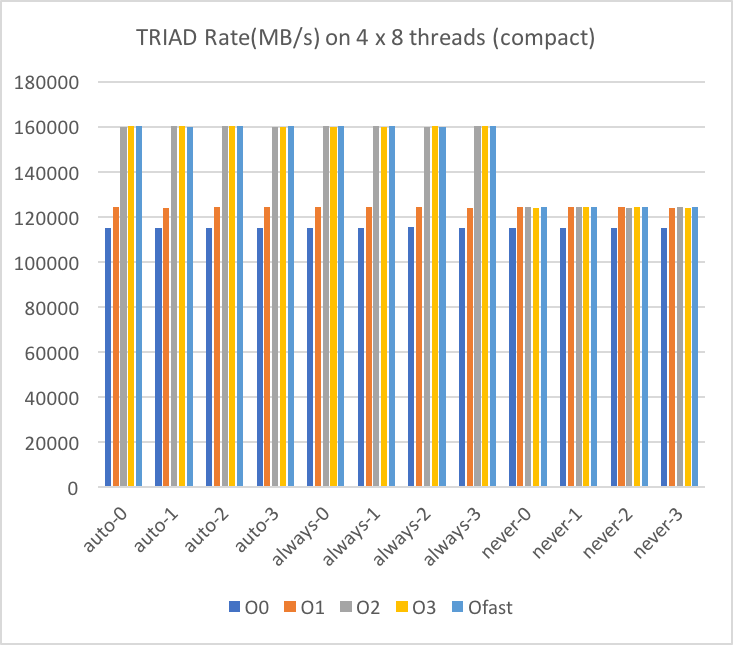
\includegraphics[width=0.45\textwidth]{figs/stream-ivy-scatter-4cpux8.png}
\caption{stream-ivy-scatter-4cpux8}
\label{fig:stream-ivy-scatter-4cpux8}
\end{figure}

これに対してアプリケーションのスレッド並列度が低い場合は様子が変わり,
例えばCPUあたり2スレッド(2コア)が実行されると
図\ref{fig:stream-ivy-scatter-4cpux2} の様になる.\\

\begin{figure}[bt]
\centering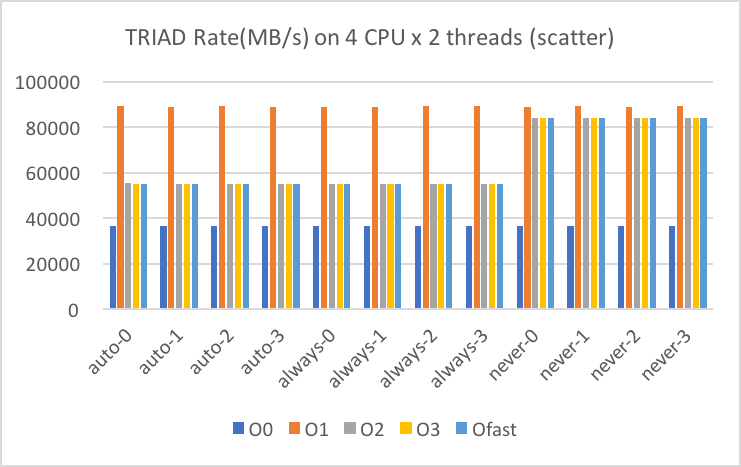
\includegraphics[width=0.45\textwidth]{figs/stream-ivy-scatter-4cpux2.png}
\caption{stream-ivy-scatter-4cpux2}
\label{fig:stream-ivy-scatter-4cpux2}
\end{figure}

図\ref{fig:stream-ivy-compact-1cpux8} と
図\ref{fig:stream-ivy-scatter-4cpux2} と
でPMlibが出力するHWPC Cache関係の数値を比較すると***
が読み取れる.
\fi


\section{謝辞}
本論文の一部は,文部科学省「特定先端大型研究施設運営費等補助金(次世代超高速電子計算機システムの開発・整備等)」で実施された内容に基づくものである.

%\cite{webpage2} \par
%\cite{webpage3} \par

\bibliographystyle{jplain}
\bibliography{main}
%\bibliography{bibsample}
\end{document}

